\section{$\mu^+\to e^+\gamma$}

Recent MEG measurement at PSI~\cite{MEG2013} sets a limit of 
${\cal B}(\mu^+\to e^+\gamma)< 5.7\times 10^{-13}$ at 90\% confidence
level using $3.6\times 10^{14}$ stopped muons on target. The MEG detector
consists of a set of drift chambers and scintillation timing counters,
located inside a superconducting solenoid, and a liquid Xenon 
calorimeter with UV-sensitive photomultiplier tubes, located outside the
solenoid. 

There are two main sources of background. Over 90\% of the background in
the signal region comes from accidental background, that is, a positron
from a regular Michel muon decay combined with a photon from a radiative
muon decay  (RMD) $\mu^+\to e^+ \nu_e\bar\nu_\mu \gamma$.
Most of the remainig background is RMD where the neutrinos carry away minimum
energy. The accidental background rate depends on instantaneous stopping
muon rate $R_\mu$, total integrating data acquisition time $T$, and 
detector resolutions:
\begin{equation}
N_{\rm acc} \propto R_\mu^2 \times \Delta E_\gamma^2 \times\Delta P_e \times
\Delta \Theta_{e\gamma}^2 \times \Delta t_{e \gamma} \times T, 
\end{equation}
where $\Delta E_\gamma$ and $\Delta P_e$ are the resolutions of photon energy
and positron momentum, respectively; $\Delta \Theta_{e\gamma}$ and
$\Delta t_{e \gamma}$ are the resolutions of $e\gamma$ opening angle and
timing.

MEG Collaboration has proposed an upgrade~\cite{MEGupgrade} aiming to 
improve the sensitivity to be able to detect $\mu\to e\gamma$ decay 
at one order of magnitude below the current limit, or set a limit at
$\sim 6\times 10^{-14}$ in the absence of signal. They will replace 
their tracker with a lower-mass, higher-granularity device, reduce target
thickness, use a faster timing counter array, and increase the 
granularity of the liquid xenon detector by replacing the PMTs with 
a larger number of smaller solid state photo sensors. The sensitivity
estimate is based on a muon stopping rate of $7\times 10^7$ muons/s for 
a 3-year run, assuming 180 DAQ days per year.



To go beyond MEG upgrade, one needs to further improve the detector 
sensitivity. 
The photon energy resolution is a major limiting factor in this search.
A pair spectrometer that measures $e^+e^-$ pair tracks from photon
conversions at a thin dense material can greatly improve the photon energy
resolution. The lost of efficiency due to limited photon conversion 
probability can be compensated by higher beam power that Project X at 
Fermilab could deliver, and by the increase of fiducial coverage. 

We have conducted an initial study of this concept using a fast simulation
tool (FastSim) originally developed for the Super$B$ experiment~\cite{SuperB}
using the \babar\
software framework and analysis tools. FastSim allows us to model detector 
components as two-dimensional shells of simple geometries. Particle scattering,
energy loss, secondary particle production (due to Compton scattering, 
Bremsstrahlung, conversion, EM or hadron showers, etc.) are simulated at the
intersection of particles with detector shells. Tracks are reconstructed with
a Kalman filter into piece-wise trajectories.

The FastSim model in this study consists of a thin aluminum stopping target 
and a six-layer
cylindrical silicon detector. A 0.56 mm thick lead (10\% $X_0$) half cylinder 
covering 0--$\pi$ in azimuthal angle at $R = 80$ mm serves as the photon converter.
The target consists of two cones connected at their base; each cone is 50 mm 
high, 5 mm in radius, and 50 $\mu$m thick. Two silicon detector cylinders are
placed close the target for better vertexing resolution; two layers are placed
just outside the Pb converter, and two layers a few cm away. The layout is shown
in Fig.\ref{fig:detscheme}, and a signal event display is shown in 
Fig.~\ref{fig:evtdisplay}. The entire detector is placed in a 1-T solenoidal
magnetic field.


\begin{figure}[htbp]
\centering
\begin{minipage}[c]{0.47\textwidth}
\centering
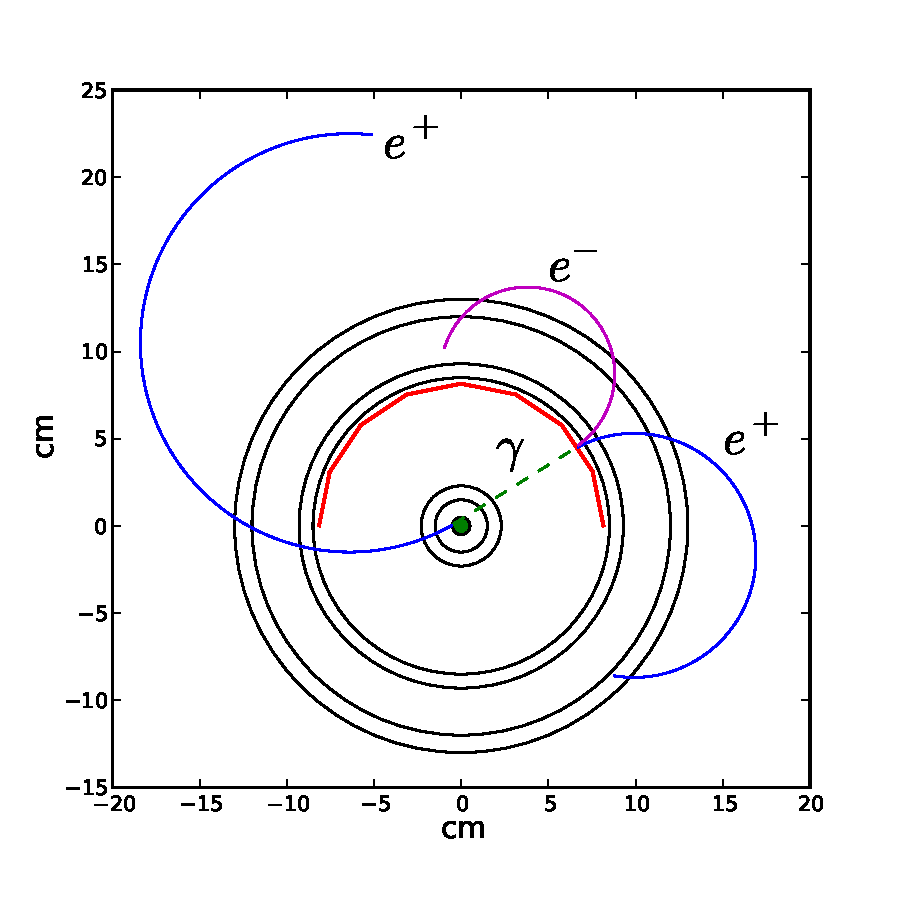
\includegraphics[width=\textwidth]{Figures/muegamma-schematic.pdf}
\caption{Schematic drawing ($x$-$y$ view) of the $\mu\to e\gamma$ detector.}
\label{fig:detscheme}
\end{minipage}
\quad
\begin{minipage}[c]{0.47\textwidth}
\centering
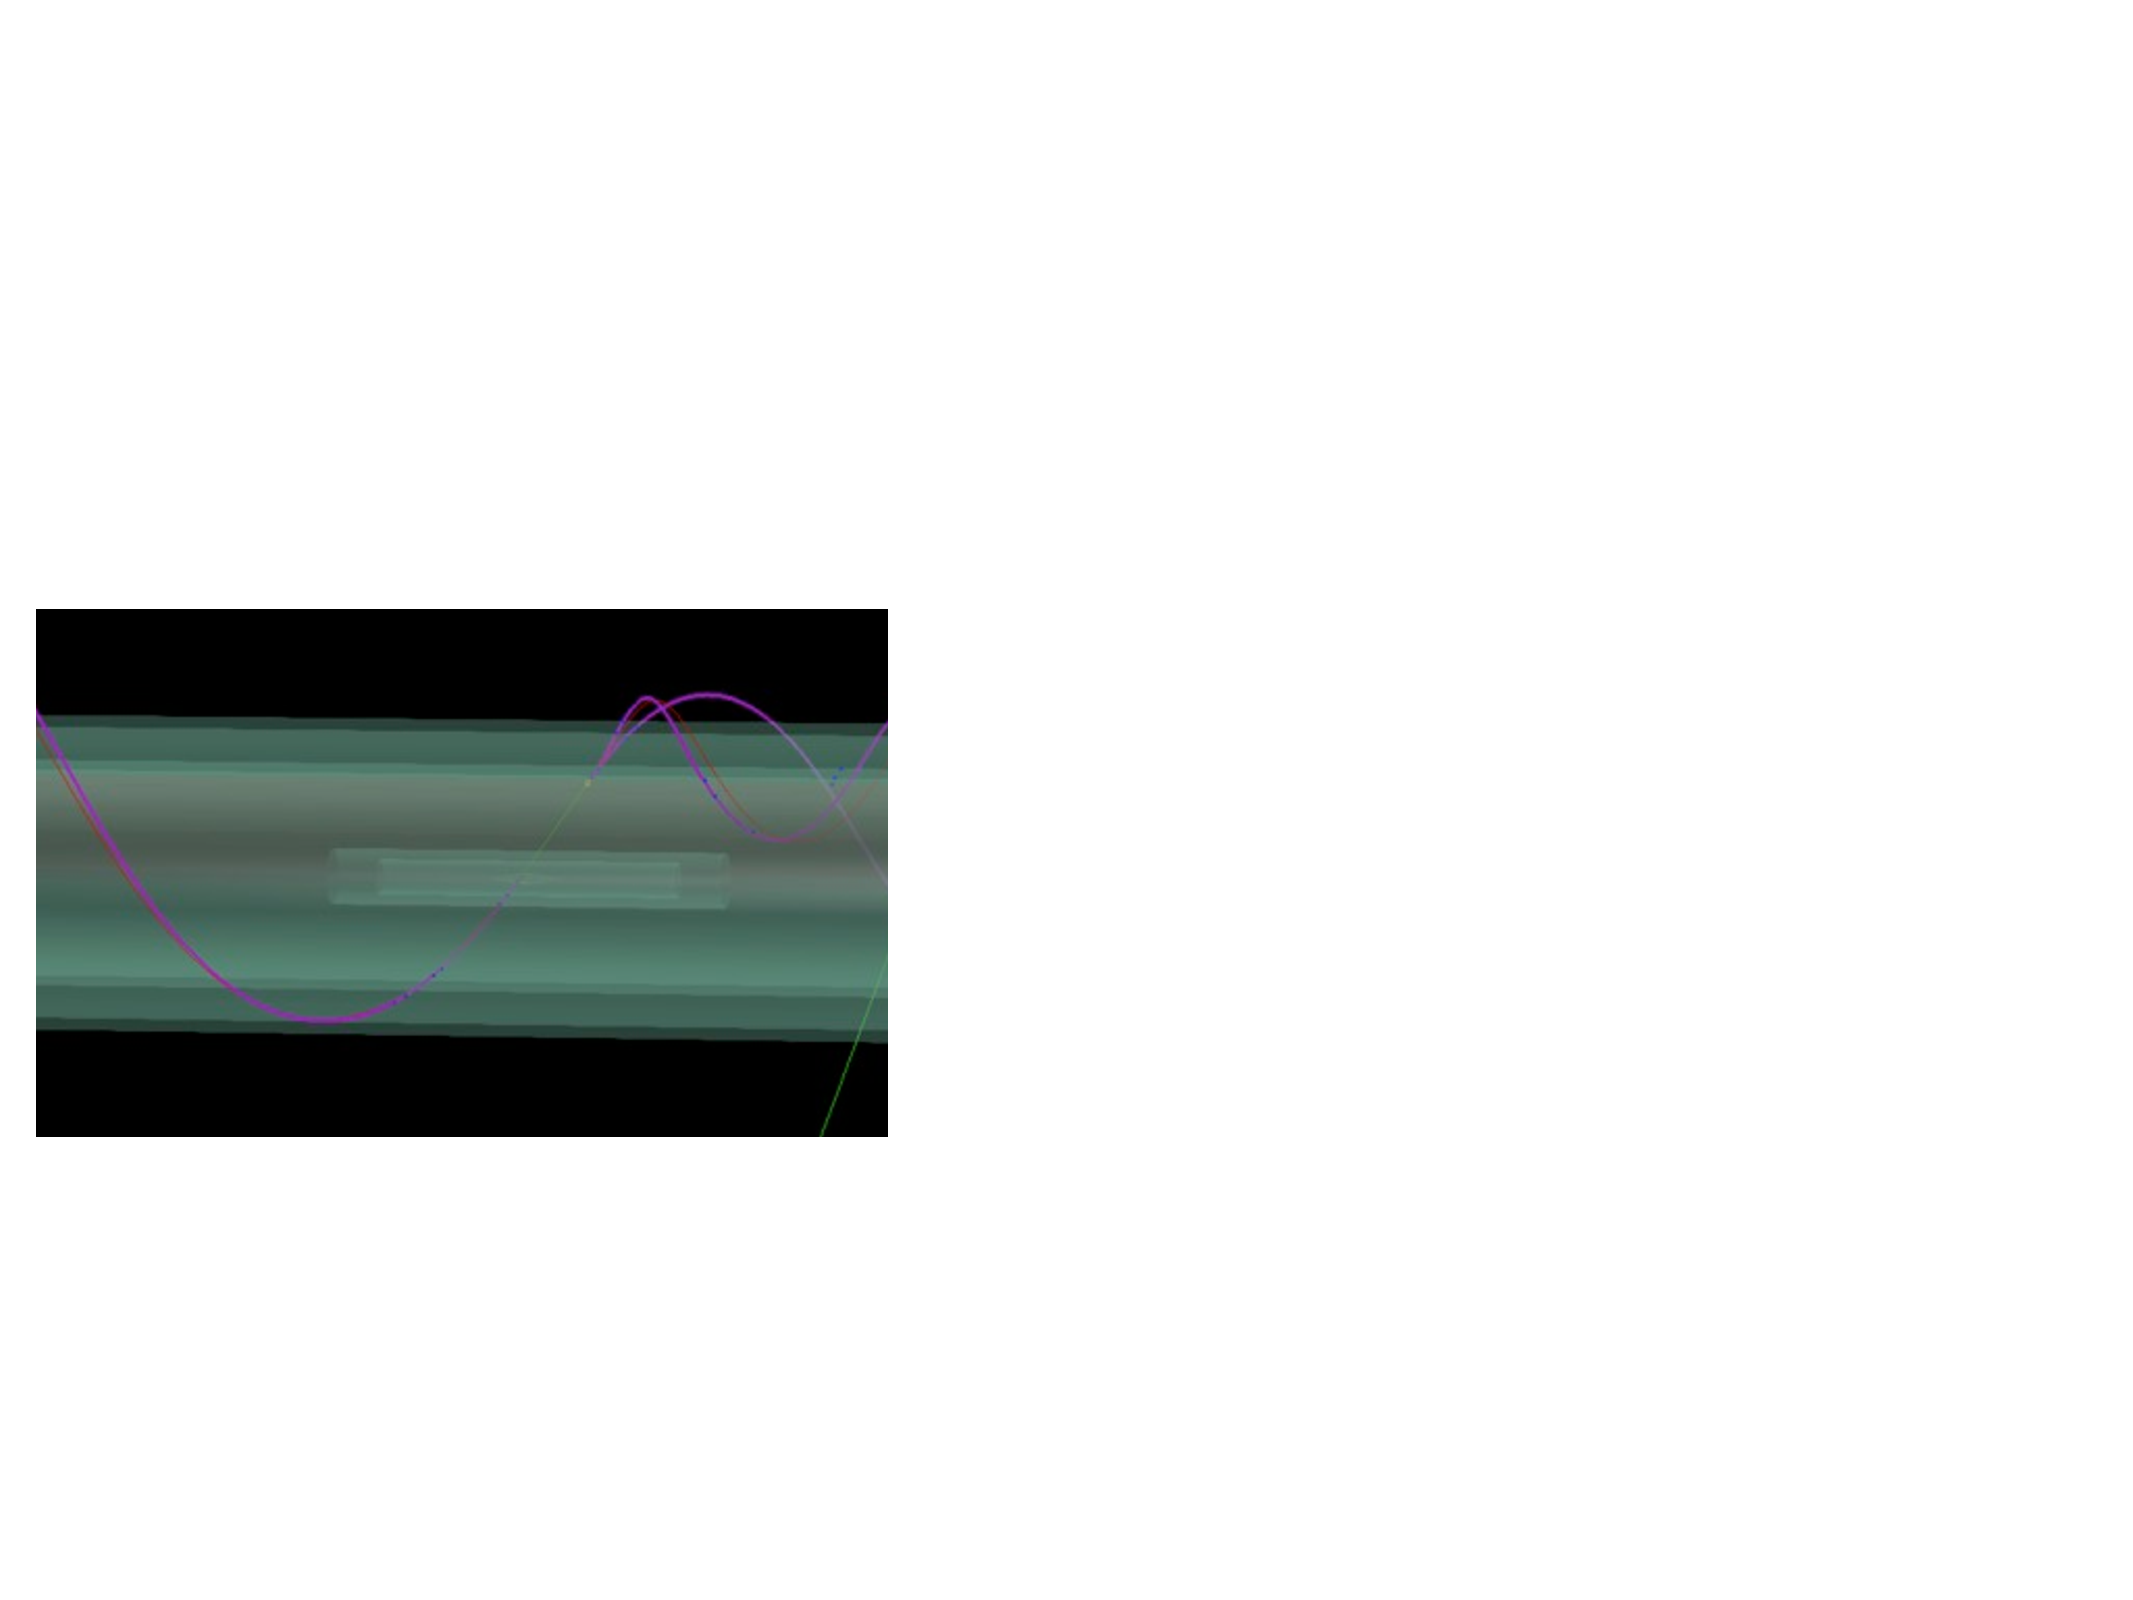
\includegraphics[width=\textwidth]{Figures/event_display.pdf}
\caption{FastSim signal event display}
\label{fig:evtdisplay}
\end{minipage}
\end{figure}

We generate muons at rest and let them decay via $\mu^+\to e^+\gamma$
to study the reconstruction efficiency and resolution. 
Approximately 1.3\% of generated signal events are well-reconstructed, 
passing quality and fiducial selections criteria. The photon energy resolution 
is approximately 200~keV (Fig.~\ref{fig:eresol}), similar to the positron momentum
resolution, which 
corresponds to 0.37\% for 52.8 MeV photons. This is a great improvement compared 
to the 1.7\%--2.4\% resolution of the current MEG and the 1.0\%--1.1\% resolution 
goal of the MEG upgrade. 

\begin{figure}[ht]
\centering
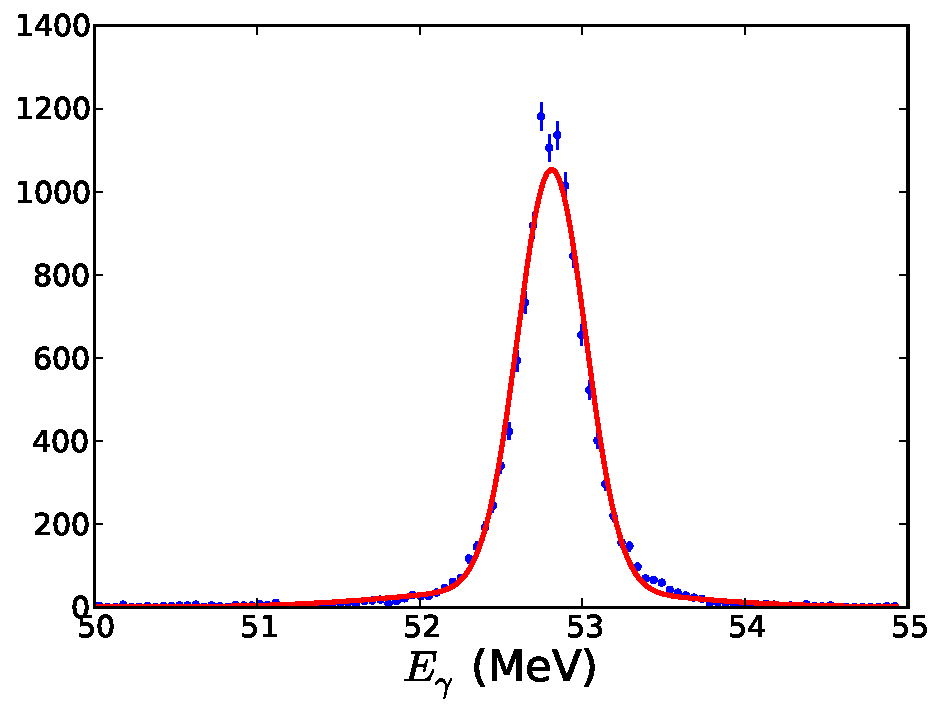
\includegraphics[width=0.49\textwidth]{Figures/egamma-resol-fit2b.pdf}
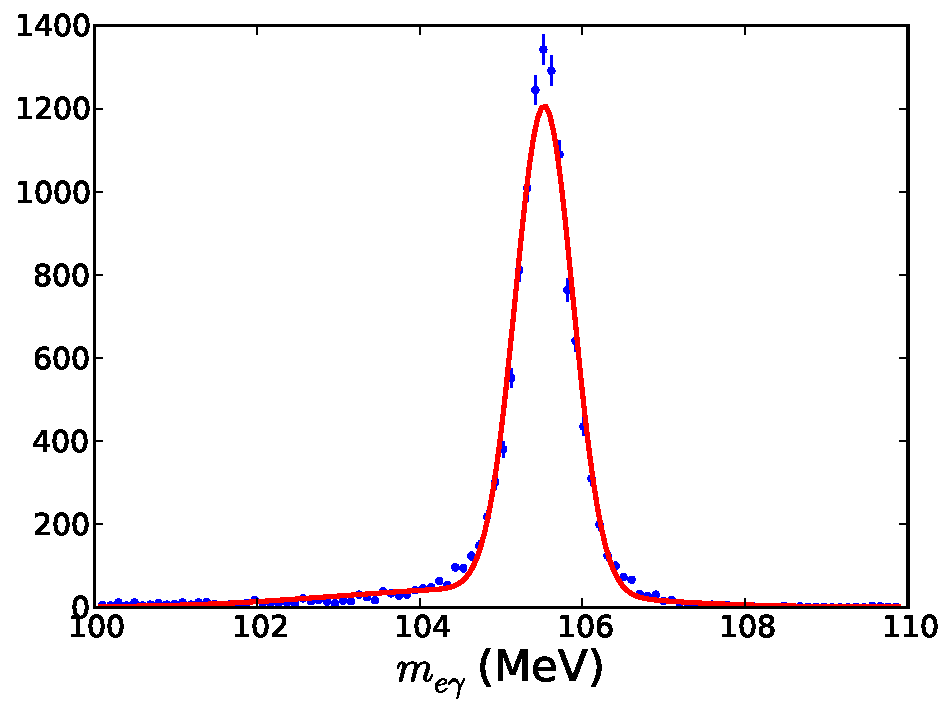
\includegraphics[width=0.49\textwidth]{Figures/mumass-resol-fit2b.pdf}
\caption{\label{fig:eresol} Photon energy resolution and $e\gamma$ invariant
mass resolution. Fitted curve is a double-Gaussian distribution.}
\end{figure}


The positron angular resolution is slightly below 10~mrad in both $\theta$ 
and $\phi$ views,
better than current MEG performance but worse than MEG upgrade projection.
The photon direction determined solely from $e^+e^-$ momenta has a resolution
similar to that of the positron. It can be further improved  by using
vertex information. Both $\gamma\to e^+e^-$ vertex and positron production vertex
(by extrapolating positron track back to the target) have a position resolution
of the order of 100~$\mu$m. Therefore, the photon direction (by connecting two
vertices) has a resolution of the order of 1~mrad (given the lever arm of 80 mm).
As a result, the resolution of the angle between $e^+$ and $\gamma$ is dominated
by $e^+$ angular resolution.

We then use a toy Monte Carlo technique to test the sensitivity of this
apparatus.
For accidental background, we generate $e^+$ and $\gamma$ from Michel
spectrum and RMD spectrum~\cite{Kuno:1999jp}, respectively. Only those 
near the end points of the spectra could contribute to the background.
The directions, production points, and production times of $e^+$ and 
$\gamma$ are generated
randomly without correlation. We ignore the other $e^+$ from the RMD that
contribute the $\gamma$.
For RMD background, we generate $e^+$ and $\gamma$ according to theoretical
partial branching fraction formula~\cite{Kuno:1999jp}. Their directions are
correlated, and their production times and positions are identical.
The number of accidental background is a product of $R_\mu^2$, partial
branching fractions of Michel decay and RMD, selection timing window,
total DAQ time, phase space factors, and reconstruction and selection 
efficiencies. For RMD background, the scaling factor is $R_\mu$, instead of
$R_\mu^2$.

The momenta 
of $e^+$ and $\gamma$ are smeared according to the FastSim study. 
We study the scenarios where the timing resolution is 50~ps and 100~ps. 
MEG experiment uses 5 independent variables $E_\gamma$, $p_e$, 
$\phi_{e\gamma}$, $\theta_{e\gamma}$, and $\Delta t_{e\gamma}$, to construct
their likelihood function. In our detector, we can take advantage of excellent
direction resolution of the converted photon. If the $\gamma$ is produced
at a different point from $e^+$ production point, as in accidental background,
 the direction of the $\gamma\to e^+e^-$ momentum and that of the line
connecting $e^+e^-$ vertex and primary $e^+$ production point on the target
will be different. So two additional variables $\Delta\theta_\gamma$ 
and $\Delta\phi_\gamma$ are used in our study. The comparisons between signal
and accidental background are shown in Fig.~\ref{fig:muegamma-vars}.

To estimate the 90\% C.L. upper limit sensitivity, we use a cut-and-count
approach to estimate background level and then use Feldman-Cousins 
method~\cite{Feldman:1997qc} to calculate upper limit sensitivity assuming
no signal events are present.



\begin{figure}[htbp]
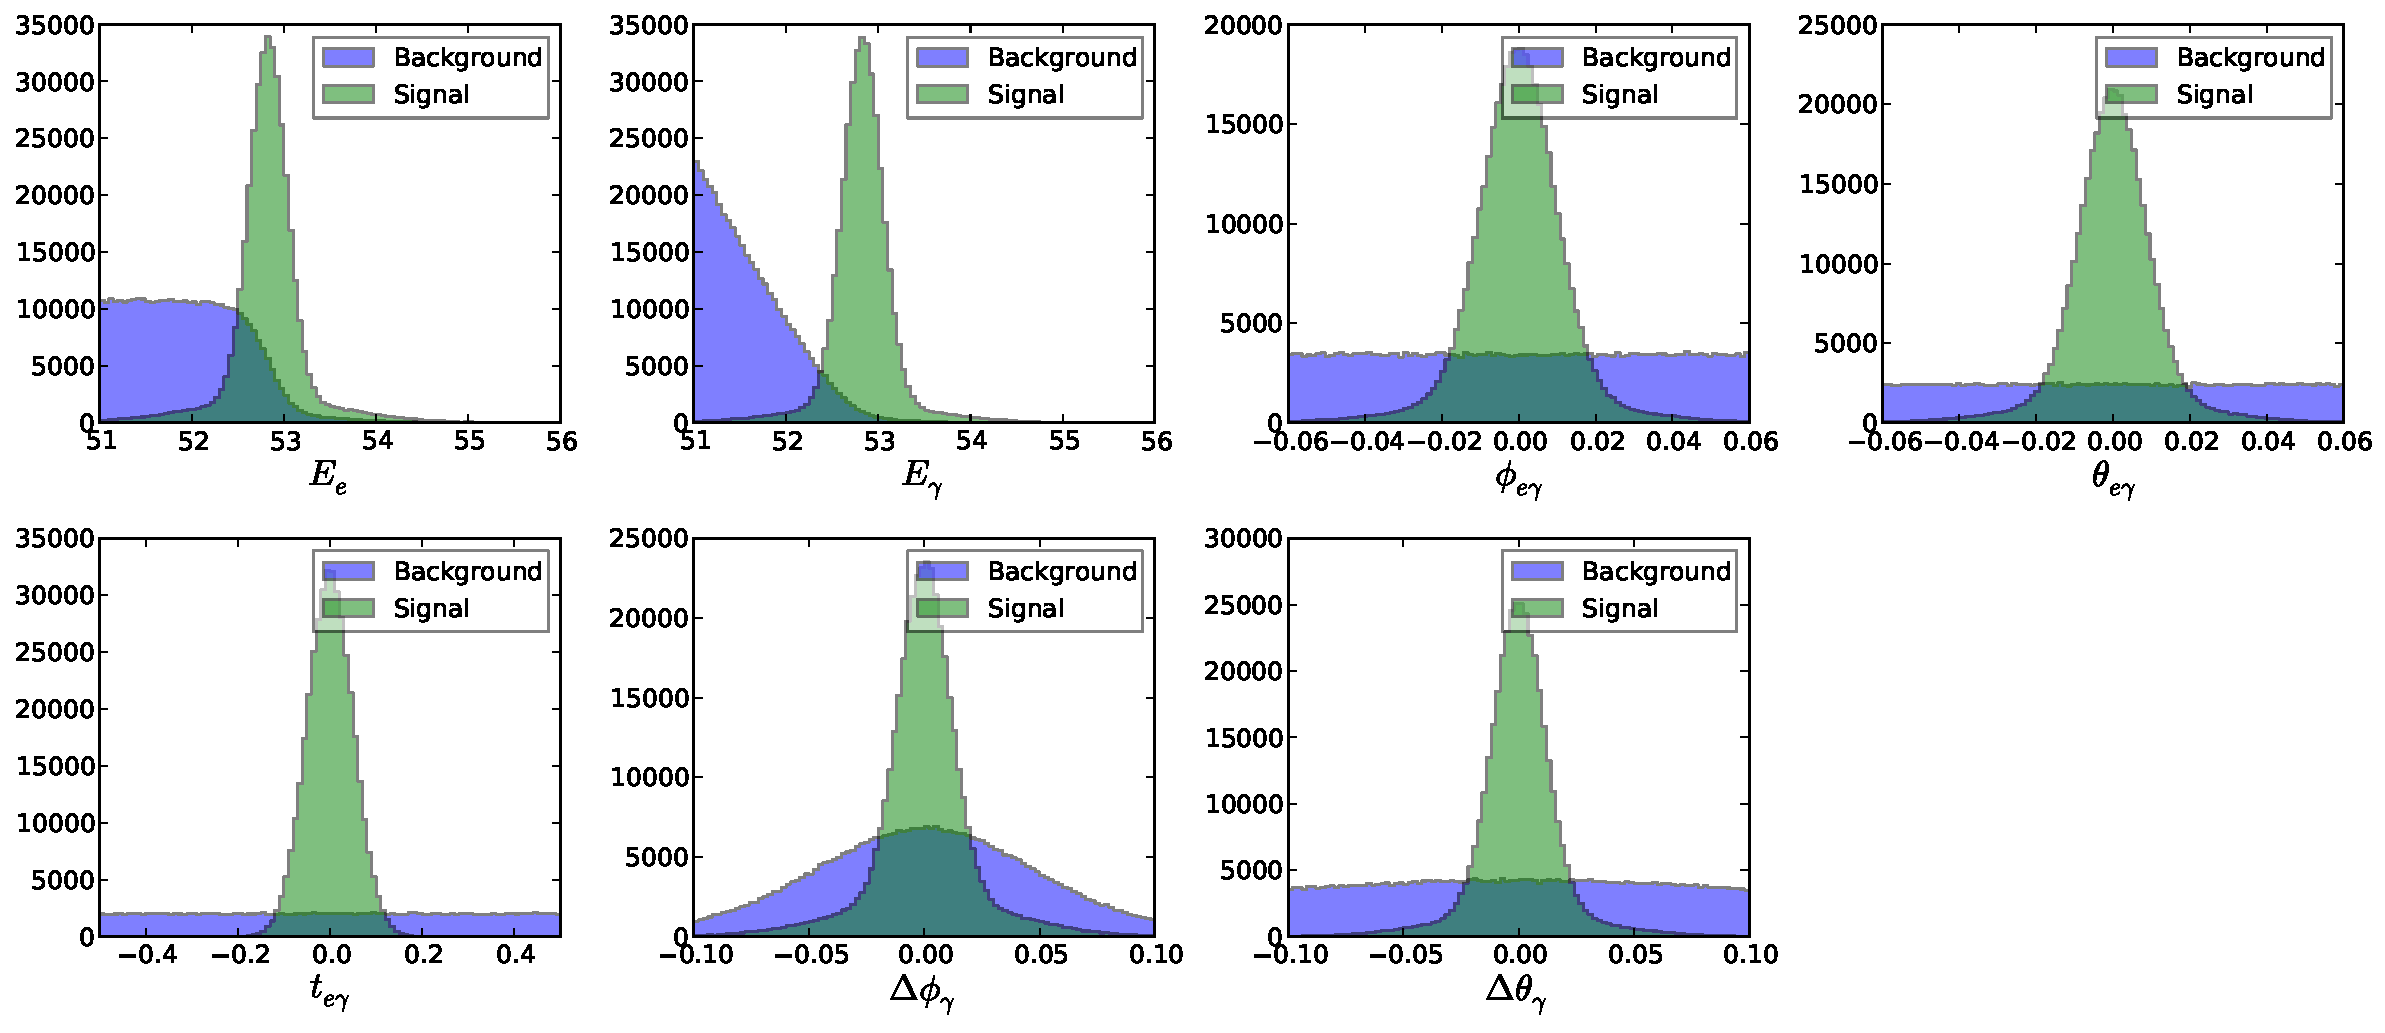
\includegraphics[width=0.99\textwidth]{Figures/sens-vardists-50ps.pdf}
\caption{Discriminating variables in $\mu^+\to e^+\gamma$ search.}
\label{fig:muegamma-vars}
\end{figure}

